\documentclass[12pt]{article}
\usepackage{graphicx, float}
\usepackage[utf8]{inputenc}
\usepackage[T2A]{fontenc}
\usepackage[serbianc]{babel}
\usepackage {amsmath, amssymb, amsthm}
\graphicspath{{figures/}}

%   formatting
\usepackage[a4paper, top=1cm, bottom=1.5cm, left=2cm, right=1cm, heightrounded]{geometry}
\renewcommand{\baselinestretch}{1.15}
\setlength{\parindent}{0pt}
\setlength{\parskip}{0.8em}

\title{Дипломски Рад}
\author{Лазар Попадић}
\date{Август 2024}
%\maketitle

\begin{document}

\section{Теорија}
\subsection{Машине једносмерне струје}
Машине једносмерне струје, у наставку МЈС, су електромеханички претварачи, који улазну електричну енергију претварају у механички рад. Састоје се из статора и ротора(арматуре). Статор успоставља побудно магнетно поље, због чега се назива и побуда. Кроз ротор се, преко четкица и комутатора, пропушта улазна арматурна струја. По принципу Лоренцовог закона $\vec F=Q(\vec v \times \vec B)$, индукује се сила која делује на ротор. Комутатор врши промену смера арматурне струје у зависности од положаја ротора, и тиме омогућава да Лоренцова сила увек делује у истом смеру, односно обезбеђује константан обртни момент мотора. Због Фарадејевог закона и Ленцовог правила $e_a=-N\dfrac{\partial\phi }{\partial t}$, обртање ротора индукује електромоторну силу супротног смера.

\begin{figure}[H]
    \centering
    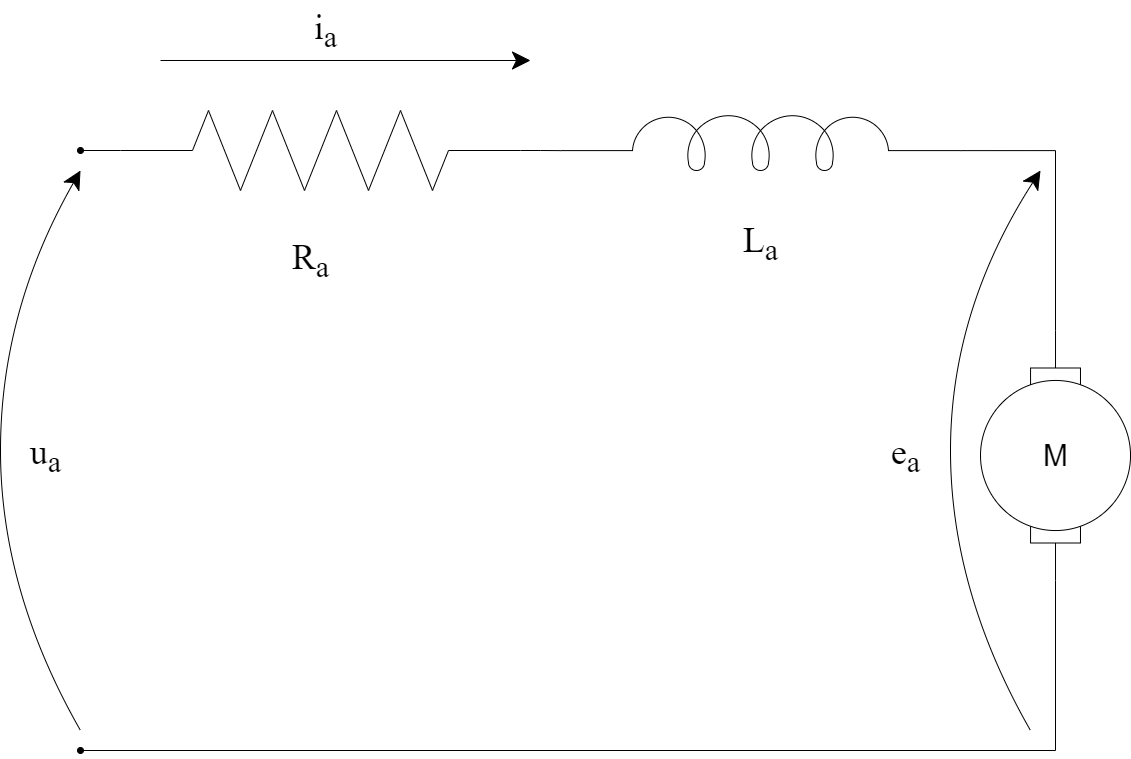
\includegraphics[width=10cm]{figures/ekv_kolo_armatura.png}
    \caption{Еквивалентно коло арматуре МЈС}
    \label{fig:коло_арматуре}
\end{figure}

\subsubsection{Динамички модел МЈС}
Модел МЈС се састоји из 2 подсистема: механичког и електричног, који међусобно интерагују. Посматраћемо МЈС која има сталну побуду јачинe магнетног флукса $\psi _f$. Модел се састоји из 3 диференцијалне једначине: напонске равнотеже арматурног навоја, механичке равнотеже и релације механичке брзине обртања и угла ротора. Као и из 2 алгебарске једначине: дефиниције електромагнетног момента и дефиниције индуковане електромоторне силе.
\begin{equation}
    u_a-e_a=R_ai_a+L_a\dfrac{di_a}{dt}
\end{equation}
\begin{equation}
    m_e-m_m=J_m \dot\omega+B_m\omega
\end{equation}
\begin{equation}
    \dfrac{d\theta}{dt}=\omega
\end{equation}
\begin{equation}
    m_e=\psi _fi_a
\end{equation}
\begin{equation}
    e_a=\psi _f\omega
\end{equation}
Значења величина математичког модела МЈС:
\begin{itemize}
    \item $u_a$ - улазни арматурни напон
    \item $e_a$ - индукована електромоторна сила
    \item $R_a$ - електрична отпорност арматурног намотаја
    \item $i_a$ - арматурна струја
    \item $L_a$ - индуктивност арматурног намотаја
    \item $m_e$ - електромагнетни моменат
    \item $m_m$ - моменат оптерећења погона
    \item $J_m$ - моменат инерције обртних маса
    \item $\omega$ - угаона брзина арматуре
    \item $B_m$ - коефицијент пригушења брзине услед трења
    \item $\theta$ - угао ротора
    \item $\psi _f$ - јачина магнетног флукса побуде
\end{itemize}

\subsubsection{МЈС у стационарном стању}
Стационарно стање МЈС подразумева режим рада у којем су изводи променљивих стања по времену једнаки нули. Односно, арматурни напон и струја, моменат оптерећења и угаона брзина су константни. Овакво стање система је равнотежно и омогућава нам да лакше увидимо законитости утицаја улазних величина на излазне. Из једначина (2) и (4) следи:
\begin{equation}
    i_a=\dfrac{B_m\omega+m_M}{\psi _f}
\end{equation}
Уврштавањем (5) и (6) у (1):
\begin{equation}
    \omega(1+\dfrac{R_aB_m}{\psi _f^2})=\dfrac{u_a}{\psi _f}-\dfrac{R_am_m}{\psi _f^2}
\end{equation}
Из (7) се може закључити да повећањем арматурног напона, угаона брзина линеарно расте, а повећањем момента оптерећења угаона брзина линеарно опада. Из тог закључка следи и идеја о регулацији брзине МЈС променом улазног арматурног напона.

\begin{figure}[H]
    \centering
    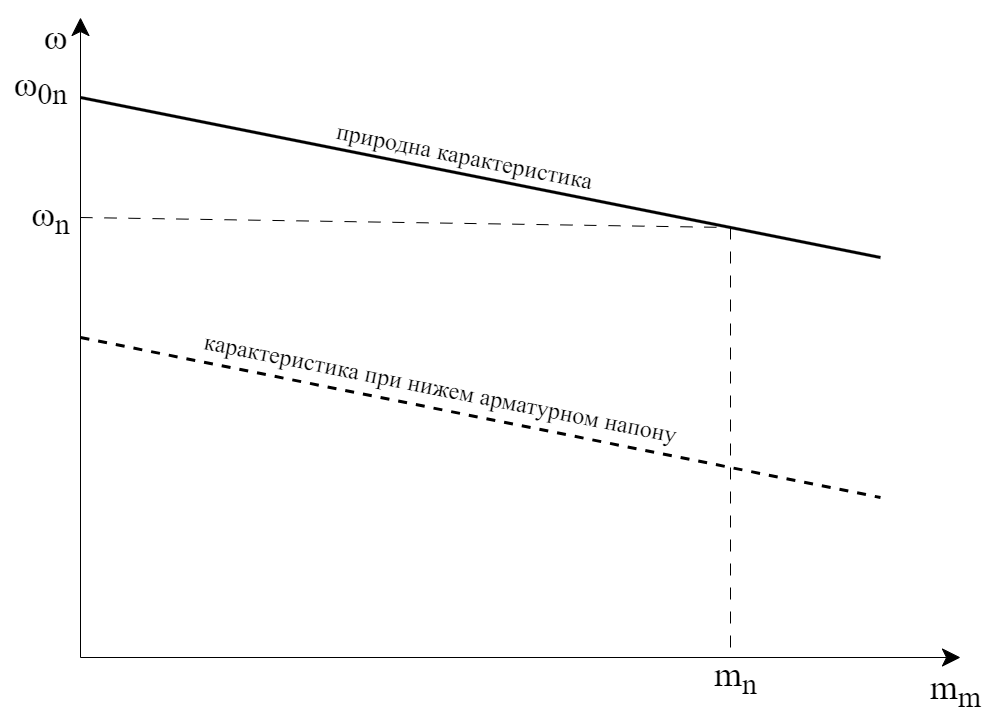
\includegraphics[width=12cm]{figures/k-ka_bdc.drawio.png}
    \caption{Механичка карактеристика МЈС}
    \label{fig:карактеристика_мјс}
\end{figure}

\end{document}
